\documentclass[11pt,a4paper]{article}
\usepackage{geometry}
\geometry{top=2.5cm, bottom=2.5cm, left=2.5cm, right=2.5cm}
\usepackage{graphicx}
\usepackage{setspace}
\usepackage{tikz}
\usetikzlibrary{calc}
\usepackage{eso-pic}
\usepackage{titlesec}
\usepackage{float}
\usepackage{xcolor}
\usepackage{booktabs}
\usepackage{amsmath} % اضافه شده جهت پشتیبانی از دستور \text در فرمول‌ها

\titleformat{\section}{\fontsize{18pt}{22pt}\bfseries}{\thesection}{1em}{}
\titleformat{\subsection}{\fontsize{15pt}{19pt}\bfseries}{\thesubsection}{1em}{}

\usepackage[pagebackref=false]{hyperref}
\hypersetup{
    colorlinks=true,
    linkcolor=blue,
    citecolor=blue,
    urlcolor=blue
}

\usepackage{xepersian}
\settextfont{Arial}
\setlatintextfont{Arial}

\begin{document}

\AddToShipoutPictureBG{
    \begin{tikzpicture}[remember picture, overlay]
        \node[draw, line width=2.5pt, minimum width=\paperwidth-2cm, minimum height=\paperheight-2cm, inner sep=0pt] at (current page.center) {};
        \node[draw, line width=1.0pt, minimum width=\paperwidth-2.3cm, minimum height=\paperheight-2.3cm, inner sep=0pt] at (current page.center) {};
    \end{tikzpicture}
}

\begin{titlepage}
    \centering
    \vspace*{0.5cm}
    
\includegraphics[width=3.5cm]{images/logo.png} \\[0.6cm]
    {\fontsize{14pt}{18pt}\selectfont دانشگاه صنعتی شریف} \\[0.2cm]
    {\fontsize{14pt}{18pt}\selectfont دانشکده مهندسی کامپیوتر}

    \vspace{2.5cm}
    {\fontsize{12pt}{16pt}\selectfont عنوان آزمایش:} \\[0.5cm]
    {\fontsize{20pt}{26pt}\bfseries طراحی و پیاده‌سازی مقایسه‌کننده‌های ترکیبی و ترتیبی (آبشاری و سریال)} \\[0.4cm]
    
    \vspace{1.5cm}
    {\fontsize{12pt}{16pt}\selectfont نام درس} \\[0.4cm]
    {\fontsize{14pt}{18pt}\bfseries آزمایشگاه طراحی سیستم‌های دیجیتال}

    \vspace{1.5cm}
    {\fontsize{12pt}{16pt}\selectfont نیم‌سال ۱۴۰۴-۱۴۰۳}

    \vspace{1.5cm}
    {\fontsize{12pt}{16pt}\selectfont استاد} \\[0.4cm]
    {\fontsize{14pt}{18pt}\bfseries دکتر اجلالی}

    \vspace{1.5cm}
    {\fontsize{12pt}{16pt}\selectfont اسامی اعضای گروه\par}
    \vspace{0.4cm}
    {\fontsize{14pt}{20pt}\bfseries
    علی سلطانی - 403106092\\[0.2cm]
    یگانه کربلایی - 403106527\\[0.2cm]
    محمدمهدی مرادی - 403106681\par}

    \vfill
\end{titlepage}

\newpage
\tableofcontents
\newpage

\section{هدف آزمایش}
هدف از این آزمایش، آشنایی با نحوه پیاده‌سازی مقایسه‌کننده‌های منطقی ترکیبی و ترتیبی در زبان توصیف سخت‌افزار Verilog است. در این راستا، با توصیف جریان داده \lr{(Dataflow)} با استفاده از دستور \texttt{assign}، ساختار سلسله‌مراتبی \lr{(Hierarchical Design)} و همچنین مدل‌سازی ترتیبی بدون استفاده از بلوک‌های \texttt{always} (با استفاده از بازخورد و لچ/فلیپ‌فلاپ در سطوح انتساب پیوسته) آشنا می‌شویم.

\section{مقایسه‌کننده ۴-بیتی آبشاری \lr{(Cascadable 4-Bit Comparator)}}

\subsection{توصیف مقایسه‌کننده ۱-بیتی آبشاری}
در مقایسه‌کننده آبشاری ۱-بیتی، ۵ ورودی و ۳ خروجی داریم:
\begin{itemize}
    \item \texttt{a} و \texttt{b}: بیت‌های جاری مربوط به دو عدد ورودی.
    \item \texttt{A\_gt\_B\_in}، \texttt{A\_lt\_B\_in}، \texttt{A\_eq\_B\_in}: سیگنال‌های وضعیت حاصل از مقایسه بیت‌های پرارزش‌تر (MSB).
    \item \texttt{A\_gt\_B\_out}، \texttt{A\_lt\_B\_out}، \texttt{A\_eq\_B\_out}: سیگنال‌های خروجی وضعیت مقایسه تا بیت جاری.
\end{itemize}

معادلات منطقی حاکم بر مدار به شرح زیر است:
\begin{equation}
A_{gt\_out} = A_{gt\_in} \lor (A_{eq\_in} \land A \land \bar{B})
\end{equation}
\begin{equation}
A_{lt\_out} = A_{lt\_in} \lor (A_{eq\_in} \land \bar{A} \land B)
\end{equation}
\begin{equation}
A_{eq\_out} = A_{eq\_in} \land \overline{(A \oplus B)}
\end{equation}

کد Verilog این پیمانه در ادامه آمده است:

\begin{figure}[H]
    \centering
    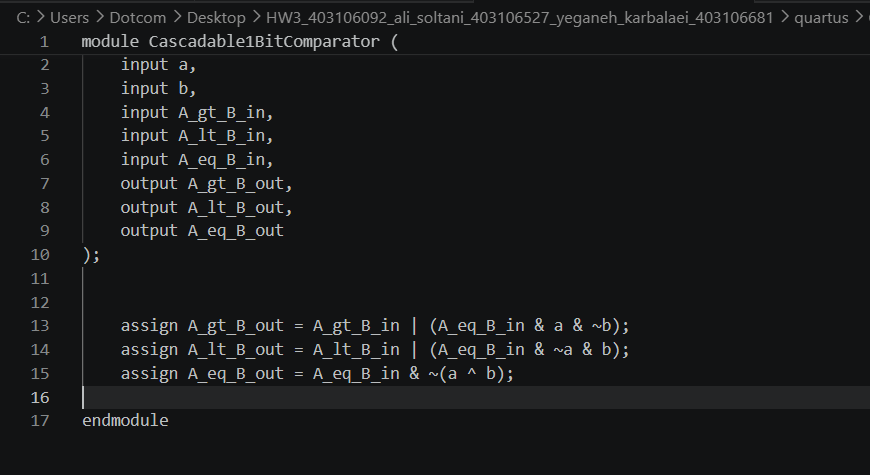
\includegraphics[width=0.85\textwidth]{images/1.png}
    \caption{کد Verilog مقایسه‌کننده ۱-بیتی آبشاری}
    \label{fig:code_1bit}
\end{figure}

\subsection{طراحی سلسله‌مراتبی مقایسه‌کننده ۴-بیتی}
با \lr{Instantiation} چهار باره از پیمانه ۱-بیتی، یک مقایسه‌کننده ۴-بیتی می‌سازیم. ورودی‌های اولیه برای باارزش‌ترین بیت (MSB) به صورت $A=B$ در نظر گرفته می‌شوند ($A_{eq\_in}=1$ و بقیه $0$). خروجی‌های هر مرحله به ورودی‌های آبشاری بیت کم‌ارزش‌تر بعدی متصل شده و خروجی مرحله آخر (LSB)، خروجی کل مدار را تشکیل می‌دهد.

\begin{figure}[H]
    \centering
    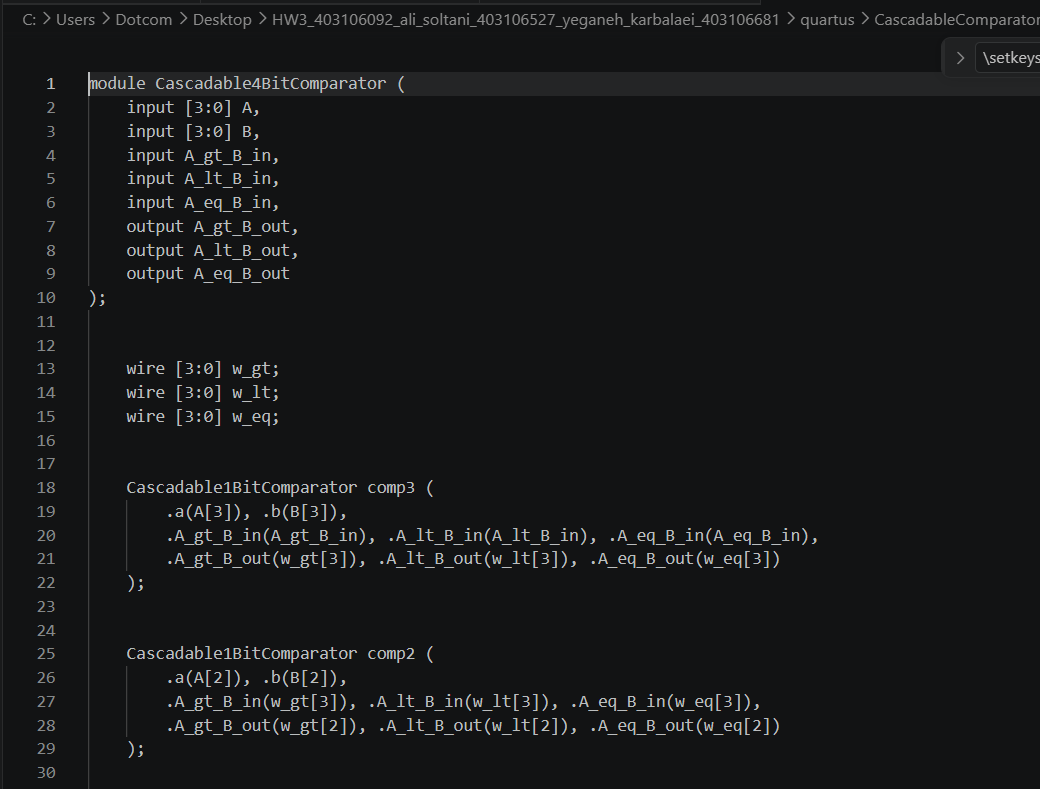
\includegraphics[width=0.85\textwidth]{images/2.png}
    \label{fig:code_4bit_1}
\end{figure}
\begin{figure}[H]
    \centering
    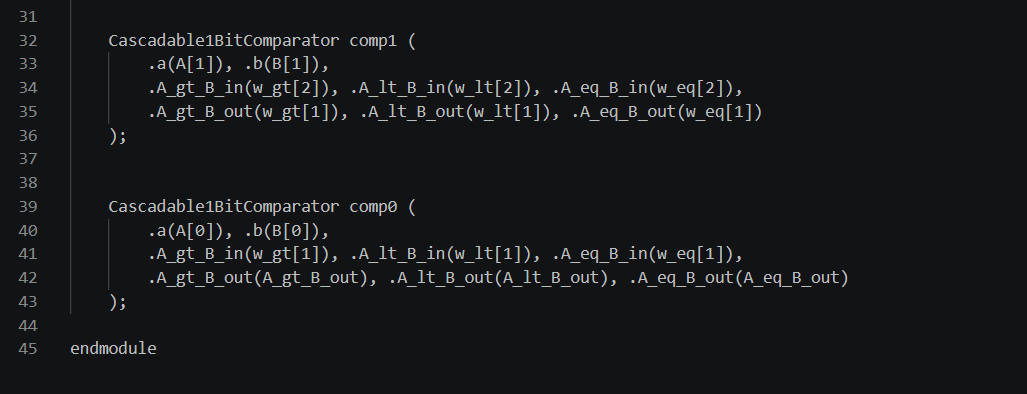
\includegraphics[width=0.85\textwidth]{images/3.png}
    \caption{کد Verilog مقایسه‌کننده ۴-بیتی آبشاری}
    \label{fig:code_4bit_2}
\end{figure}

\subsection{سنتز و دیاگرام RTL در Quartus}
طرح‌واره RTL حاصل از سنتز مدار ۴-بیتی آبشاری در نرم‌افزار Quartus نشان‌دهنده زنجیره‌سازی ۴ بلوک مقایسه‌کننده ۱-بیتی است.

\begin{figure}[H]
    \centering
    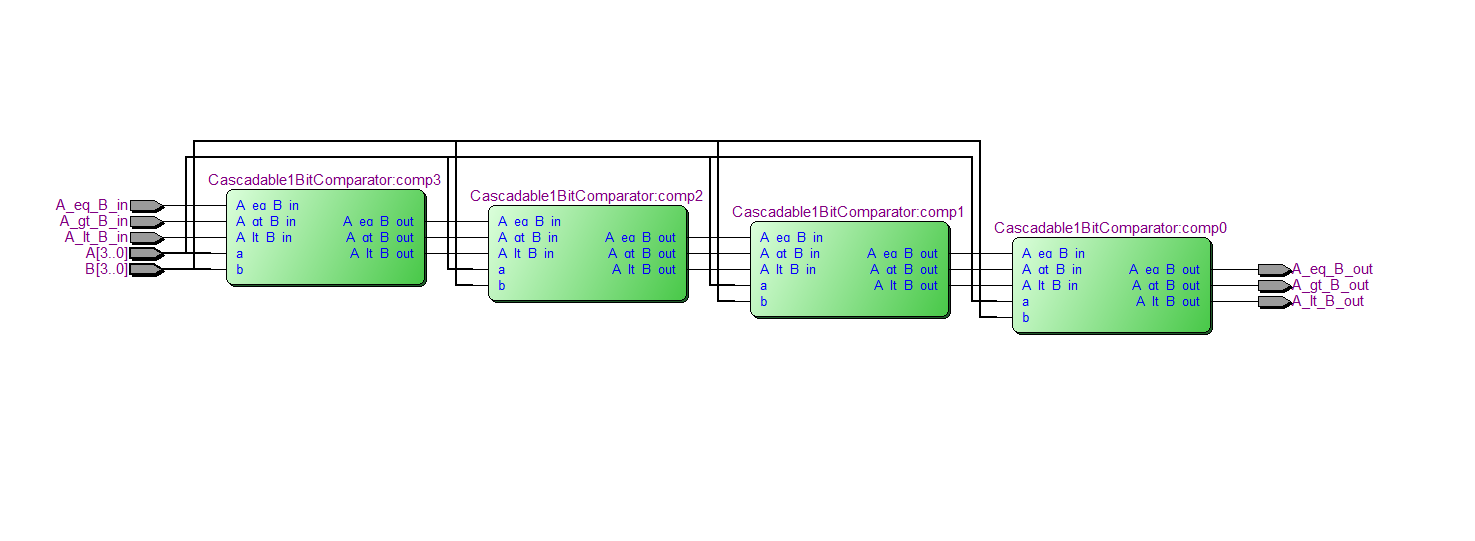
\includegraphics[width=0.85\textwidth]{images/rtl_4bit_cascaded.png}
    \caption{دیاگرام RTL مقایسه‌کننده ۴-بیتی آبشاری در Quartus}
    \label{fig:rtl_4bit}
\end{figure}

\subsection{نتایج شبیه‌سازی در ModelSim و تحلیل عملکرد}
برای تست عملکرد مدار ترکیبی، حالات متفاوتی از ورودی‌های $A$ و $B$ اعم از تساوی، بزرگتر بودن و کوچکتر بودن اعمال شدند.

\begin{figure}[H]
    \centering
    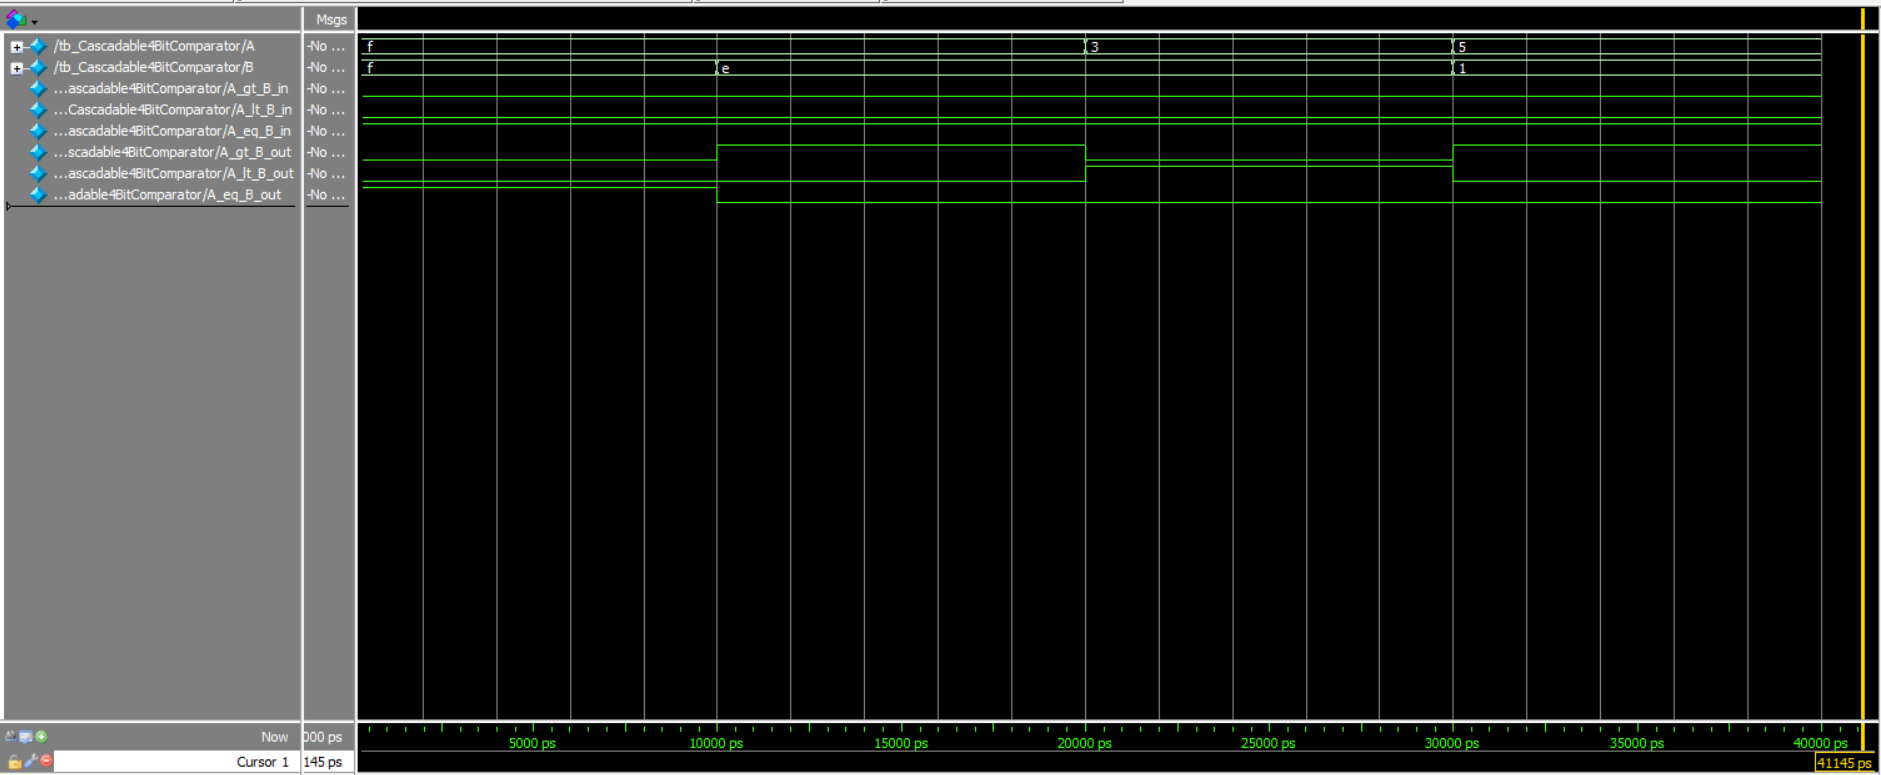
\includegraphics[width=0.95\textwidth]{images/sim_4bit_cascaded.png}
    \caption{موج‌فرم‌های شبیه‌سازی مقایسه‌کننده ۴-بیتی آبشاری در ModelSim}
    \label{fig:sim_4bit}
\end{figure}

\textbf{تحلیل موج‌فرم شبیه‌سازی:}
همان‌طور که در شکل~\ref{fig:sim_4bit} مشاهده می‌شود، به دلیل ترکیبی بودن ساختار مدار، به محض تغییر ورودی‌های $A$ و $B$، سیگنال‌های خروجی پس از گذر از تاخیر انتشار گیت‌ها \lr{(Propagation Delay)} به‌روزرسانی می‌شوند:
\begin{itemize}
    \item در بازه اولیه با اعمال $A = 15$ و $B = 15$ (حالت تساوی)، خروجی \texttt{A\_eq\_B\_out} برابر با ۱ باقی می‌ماند.
    \item با تغییر $A = 15$ و $B = 14$، از آنجا که بیت‌های MSB یکسان بوده اما در بیت LSB مقدار $A$ بزرگتر است، سیگنال \texttt{A\_gt\_B\_out} بدون نیاز به سیگنال ساعت به سطح منطقی ۱ تغییر وضعیت می‌دهد.
    \item با تغییر $A = 3$ و $B = 14$، به دلیل بزرگتر بودن $B$ در بیت‌های پرارزش، خروجی \texttt{A\_lt\_B\_out} فعال می‌شود.
\end{itemize}

\section{مقایسه‌کننده سریال \lr{(Serial Comparator)}}

\subsection{توصیف و پیاده‌سازی مدار}
مقایسه‌کننده سریال یک مدار ترتیبی است که در هر سیکل ساعت، یک جفت بیت از دو عدد را دریافت کرده و وضعیت مقایسه را به‌روزرسانی می‌کند.

کد کامل Verilog این مدار به شرح زیر است:

\begin{figure}[H]
    \centering
    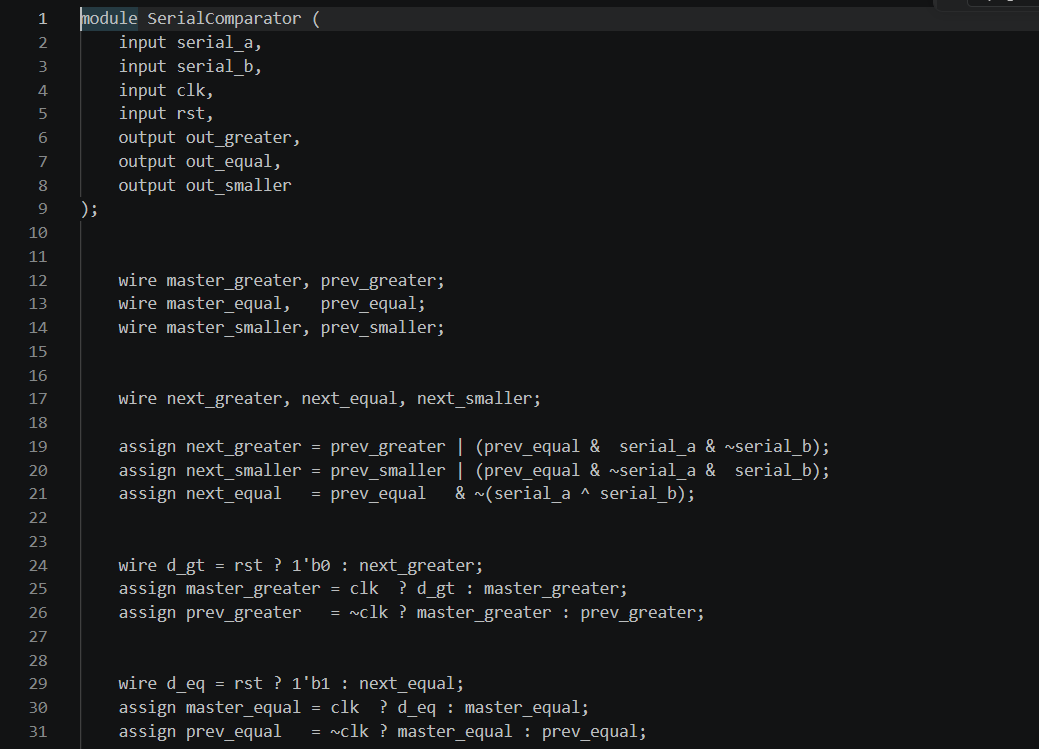
\includegraphics[width=0.85\textwidth]{images/4.png}
    \label{fig:code_serial_1}
\end{figure}
\begin{figure}[H]
    \centering
    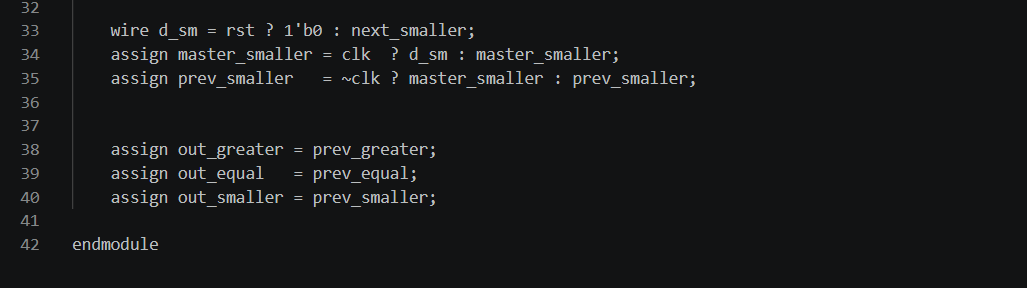
\includegraphics[width=0.85\textwidth]{images/5.png}
    \caption{کد Verilog مقایسه‌کننده سریال با دستور assign}
    \label{fig:code_serial_2}
\end{figure}

\subsection{تحلیل نحوه پیاده‌سازی فلیپ‌فلاپ Master-Slave بدون بلوک always}
در ساختارهای ترتیبی معمولاً از بلوک \texttt{always @(posedge clk)} استفاده می‌شود؛ اما بر اساس صورت آزمایش، پیاده‌سازی صرفاً با دستورات انتساب پیوسته (\texttt{assign}) انجام گرفت. برای دستیابی به رفتار حساس به لبه \lr{(Edge-Triggered)}، یک فلیپ‌فلاپ Master-Slave با استفاده از دو لچ و منطق بازخورد \lr{(Combinational Loop)} طراحی شد:

\begin{equation}
\text{\texttt{master}} = \text{\texttt{rst}} \;?\; 0 : (\text{\texttt{clk}} \;?\; \text{\texttt{master}} : \text{\texttt{cur}})
\end{equation}
\begin{equation}
\text{\texttt{prev}} = \text{\texttt{rst}} \;?\; 0 : (\sim\text{\texttt{clk}} \;?\; \text{\texttt{master}} : \text{\texttt{prev}})
\end{equation}

در این ساختار:
\begin{enumerate}
    \item هنگامی که $\text{\texttt{clk}} = 0$ است، لچ Master ورودی جدید ($\text{\texttt{cur}}$) را نمونه‌برداری کرده و شفاف \lr{(Transparent)} است، در حالی که لچ Slave حالت قبلی را حفظ می‌کند.
    \item به محض صعود سیگنال ساعت ($\text{\texttt{clk}} = 1$)، لچ Master قفل شده و ارزش ورودی روی لچ Slave منتقل می‌شود. این سازوکار رفتاری کاملاً معادل با فلیپ‌فلاپ حساس به لبه بالاارونده ایجاد می‌کند.
\end{enumerate}

\subsection{سنتز و دیاگرام RTL در Quartus}
نتیجه سنتز مدار سریال در نرم‌افزار Quartus نشان‌دهنده ایجاد ساختار لچ‌ها و گیت‌های ترکیبی مربوط به منطق حالت بعدی است.

\begin{figure}[H]
    \centering
    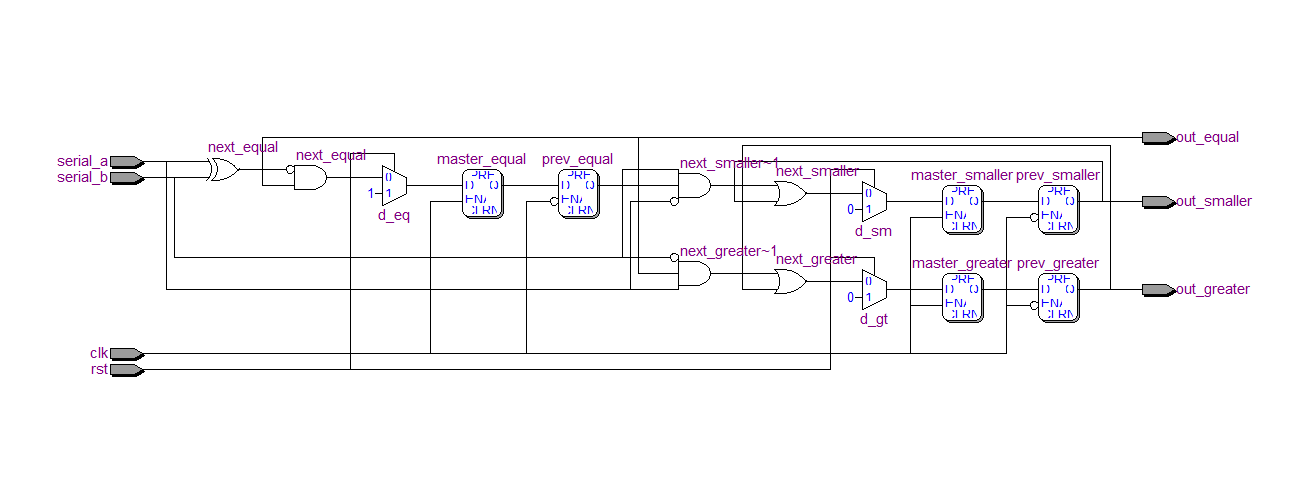
\includegraphics[width=0.85\textwidth]{images/rtl_serial.png}
    \caption{دیاگرام RTL مقایسه‌کننده سریال در Quartus}
    \label{fig:rtl_serial}
\end{figure}

\subsection{نتایج شبیه‌سازی در ModelSim و تحلیل عملکرد}
برای صحت‌سنجی مدار ترتیبی، داده‌های ورودی به صورت سری و بیت به بیت ( MSB به (LSB همگام با لبه‌های ساعت اعمال گردیدند.

\begin{figure}[H]
    \centering
    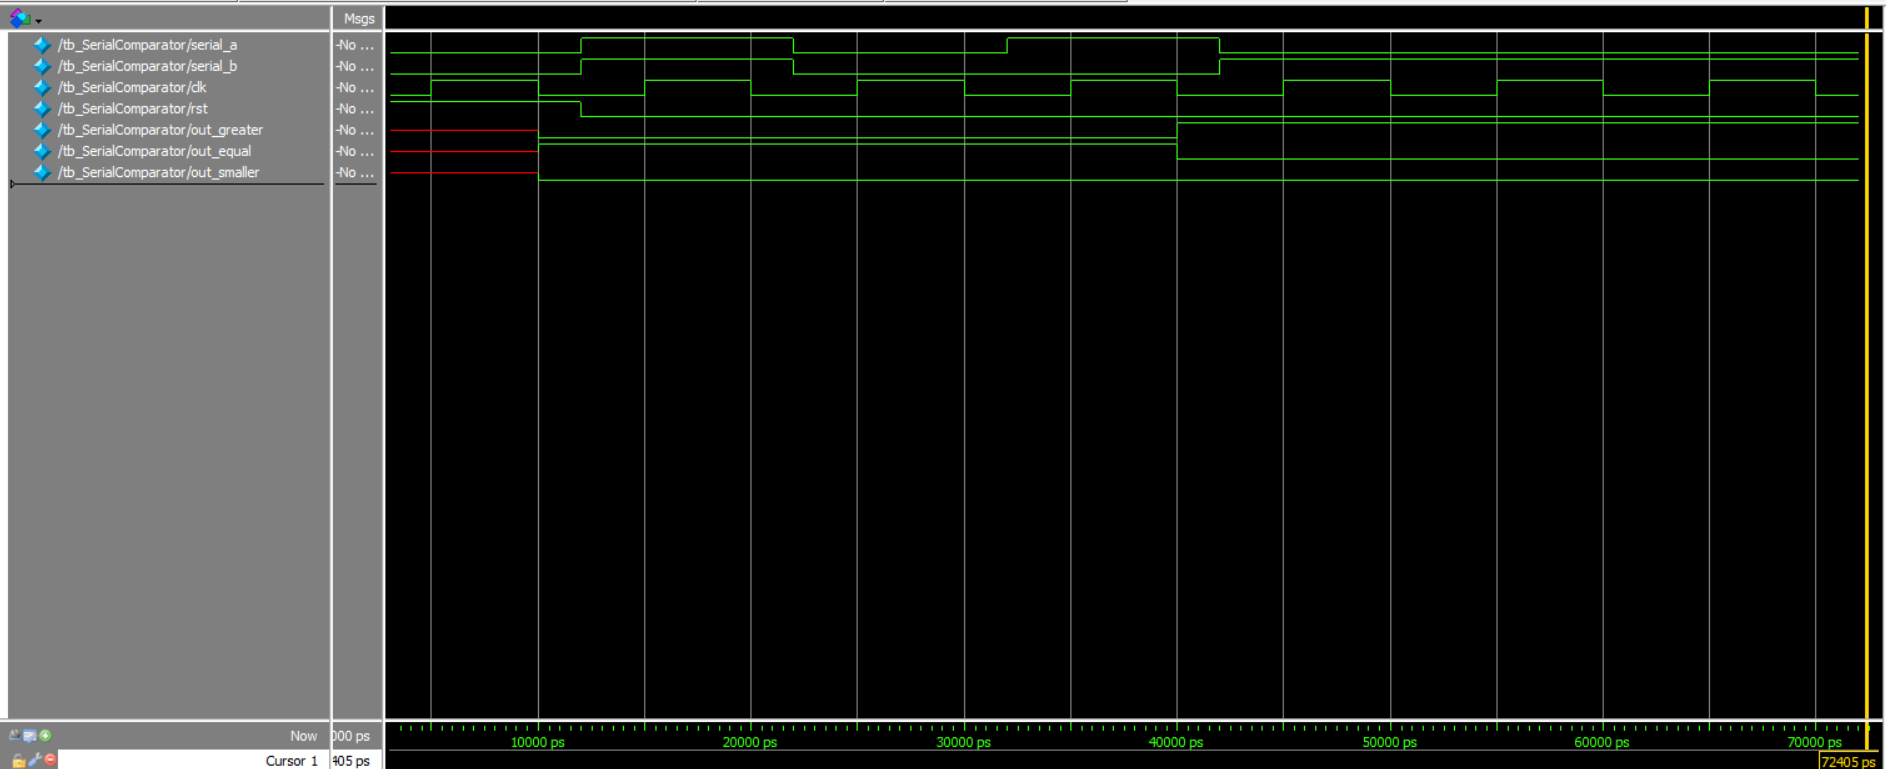
\includegraphics[width=0.95\textwidth]{images/sim_serial.png}
    \caption{موج‌فرم‌های شبیه‌سازی مقایسه‌کننده سریال در ModelSim}
    \label{fig:sim_serial}
\end{figure}

\textbf{تحلیل موج‌فرم شبیه‌سازی:}
مطابق موج‌فرم‌های شکل~\ref{fig:sim_serial}:
\begin{itemize}
    \item با فعال شدن سیگنال \texttt{rst}، تمام خروجی‌ها بازنشانی شده و سیگنال \texttt{out\_equal} به ارزش ۱ مقداردهی اولیه می‌شود.
    \item تا زمانی که بیت‌های ورودی \texttt{serial\_a} و \texttt{serial\_b} برابر باشند، وضعیت \texttt{out\_equal = 1} حفظ می‌شود.
    \item با وقوع اولین عدم تطابق در یک لبه فعال ساعت (مثلاً $\text{\texttt{serial\_a}}=1$ و $\text{\texttt{serial\_b}}=0$)، خروجی \texttt{out\_greater} فعال شده و به دلیل منطق قفل‌شوندگی \lr{(Latching Logic)}، حتی با تغییرات بعدی ورودی‌ها در سیکل‌های بعد، وضعیت تا اعمال مجدد \texttt{rst} تغییر نمیکند.
\end{itemize}

\section{مقایسه منابع سخت‌افزاری و نتیجه‌گیری}
بر اساس گزارش سنتز نرم‌افزار Quartus، میزان مصرف منابع سخت‌افزاری و ویژگی‌های عملکردی دو مدار در جدول زیر خلاصه‌سازی شده است:

\begin{table}[H]
\centering
\caption{مقایسه عملکردی و منابع سخت‌افزاری دو نوع مقایسه‌کننده}
\label{tab:comparison}
\vspace{0.3cm}
\begin{tabular}{lcc}
\toprule
\textbf{شاخص مقایسه} & \textbf{مقایسه‌کننده ۴-بیتی آبشاری} & \textbf{مقایسه‌کننده سریال} \\
\midrule
عناصر منطقی \lr{(Logic Elements / LUTs)} & رشد خطی متناسب با بیت‌ها ($O(N)$) & مقدار ثابت (مستقل از $N$) \\
ثبات‌ها/لچ‌ها \lr{(Registers / Latches)} & $0$ & $6$ عنصر حافظه Master-Slave \\
تعداد سیکل محاسبه & $1$ سیکل ترکیبی & $N$ سیکل ساعت \\
پیچیدگی سیم‌کشی \lr{(Routing)} & بالا (در بیت‌های زیاد) & بسیار کم (ورودی‌های تک‌بیتی) \\
\bottomrule
\end{tabular}
\end{table}

در نهایت، مقایسه‌کننده ترکیبی برای کاربردهایی که سرعت کارکرد بالا اولویت دارد و تعداد بیت‌ها محدود است مناسب بوده، در حالی که مقایسه‌کننده سریال برای سیستم‌های کم‌مصرف با محدودیت شدید مساحت چیپ \lr{(Silicon Area)} گزینه ایده‌آل محسوب می‌شود.

\end{document}